% =============================================================================
% FAECO 中文期刊版式（计算机辅助设计与图形学学报模板近似）
% 字体说明：模板要求方正书宋_GBK/方正仿宋_GBK/黑体/Times New Roman。
% 方正 GBK 字库为商业字体，需作者自行购买安装；当前以系统宋体/黑体/仿宋近似。
% 安装方正字库后，将下方 FZ 字体变量替换为对应方正字体名即可。
% =============================================================================
\documentclass[twocolumn,10pt,fontset=windows]{ctexart}

% -----------------------------------------------------------------------------
% 字体（方正 GBK 安装后替换此处）
%   正文:    \setCJKmainfont{方正书宋_GBK}
%   标题:    \setCJKsansfont{方正黑体_GBK}
%   仿宋:    \setCJKfamilyfont{fzfs}{方正仿宋_GBK}
% 当前用系统字体近似（fontset=windows: 宋体/黑体/楷体/仿宋）
% -----------------------------------------------------------------------------
\setmainfont[Path=./fonts/,Extension=.ttf,UprightFont=times,BoldFont=timesbd,ItalicFont=timesi,BoldItalicFont=timesbi]{Times New Roman}
\setCJKmainfont[Path=./fonts/,Extension=.ttf]{FZShuSong-Z01}
\setCJKsansfont[Path=./fonts/,Extension=.ttf]{SimHei}
\newCJKfontfamily\songfamily[Path=./fonts/,Extension=.ttf]{FZShuSong-Z01}
\newCJKfontfamily\fangfamily[Path=./fonts/,Extension=.ttf]{FZFangSong-Z02}
\newCJKfontfamily\heifamily[Path=./fonts/,Extension=.ttf]{SimHei}
\usepackage{amsmath,amssymb}
\usepackage{newtxmath}
\let\songti\songfamily\let\heiti\heifamily\let\fangsong\fangfamily
\usepackage{booktabs}
\usepackage{graphicx}
\usepackage{subfig}
\usepackage{float}
\usepackage{array}
\usepackage[nocompress]{cite}
\usepackage[hidelinks]{hyperref}
\usepackage{xurl}
\usepackage{algorithm}
\usepackage{algpseudocode}
\usepackage{multirow}
\usepackage{geometry}
\usepackage{placeins}
\usepackage{dblfloatfix}
\usepackage{balance}

% 版面：A4 双栏，栏宽 21.59 字符、栏间距 3 字符（以 3zw 近似）
\geometry{a4paper,left=2.0cm,right=2.0cm,top=2.1cm,bottom=2.1cm,columnsep=31.5pt}

\renewcommand{\eqref}[1]{\textup{（\ref{#1}）}}
\graphicspath{{../figures/}}
\setlength{\emergencystretch}{3em}
\Urlmuskip=0mu plus 3mu\relax
\raggedbottom
\setlength{\floatsep}{6pt plus 2pt minus 2pt}
\setlength{\textfloatsep}{8pt plus 2pt minus 2pt}
\setlength{\intextsep}{6pt plus 2pt minus 2pt}
\setlength{\dblfloatsep}{6pt plus 2pt minus 2pt}
\setlength{\dbltextfloatsep}{8pt plus 2pt minus 2pt}

% -----------------------------------------------------------------------------
% 标题层级（模板：1级11.5pt黑体 / 2级五号黑体 / 3级10pt书宋）
% -----------------------------------------------------------------------------
\ctexset{
  section = {format=\heiti\fontsize{11.5}{15}\selectfont, beforeskip=6pt, afterskip=4pt},
  subsection = {format=\heiti\fontsize{10.5}{14}\selectfont, beforeskip=5pt, afterskip=3pt},
  subsubsection = {format=\songti\fontsize{10}{13}\selectfont, beforeskip=4pt, afterskip=2pt}
}

% 图题（书宋9pt）、表题（黑体9pt）、表注/分图题（书宋8pt）
\usepackage{caption}
\DeclareCaptionFont{songti}{\songti}
\DeclareCaptionFont{heiti}{\heiti}
\captionsetup[figure]{font={songti,small},labelfont={bf},skip=3pt}
\captionsetup[table]{font={heiti,small},labelfont={bf},skip=3pt}
% subfig is not used in this manuscript; do not configure an unused subfloat caption.
\captionsetup{labelsep=space}

\begin{document}

\pagestyle{plain}

% -----------------------------------------------------------------------------
% 中文首部：标题/作者/单位/摘要/关键词/中图法分类号/DOI
\twocolumn[
\vspace*{-0.25cm}
\begin{center}
{\heiti\zihao{3} FAECO：面向预布局门级时序 ECO 的结构化候选搜索与失效归因}\par
\vspace{6pt}
{\fangsong\zihao{4} 佟亚龙、刘畅}\par
\vspace{4pt}
{\songti\fontsize{8}{12}\selectfont（国防科技大学计算机学院，长沙 410073）}\par\vspace{2pt}
{\songti\fontsize{8}{12}\selectfont E-mail：chancews@qq.com（通信作者）}\par
\vspace{6pt}
\end{center}
\begin{flushleft}
  {\heiti\fontsize{8.5}{13}\selectfont 摘\quad 要：}{\songti\fontsize{8.5}{13}\selectfont 预布局阶段的时序 ECO 是芯片设计中的关键环节，但可用的合法修改手段有限，候选空间大、逐次验证代价高。为此提出结构化候选搜索与失效归因框架 FAECO：围绕违例路径的局部逻辑，按多种结构特征构造修改候选并统一排序，以扩展有效候选空间；将候选失效归纳为若干类型，用于诊断搜索过程并引导后续控制；候选按轮提交，并依次通过时序分析与等价性检查验证。在 ISCAS89、ITC-99 与 PicoRV32 三个公开基准上，分别有 8/8、18/19 与 2/3 个实例取得时序改善，且无实例退化（尚未达到完全时序收敛）；固定配置下，混合类型候选平均改善 1.07\,ns，明显高于仅门尺寸调整的 0.16\,ns。实验还表明，单纯降低逻辑深度未必带来时序收益，说明该阶段的优化目标应以时序指标为准。}
\par
\vspace{4pt}
{\heiti\fontsize{8.5}{13}\selectfont 关键词：}{\songti\fontsize{8.5}{13}\selectfont 时序 ECO；门级局部重构；多特征加权割；类型化失效归因；分层验证；预布局时序优化}\par
\vspace{2pt}
{\songti\fontsize{8.5}{13}\selectfont 中图法分类号：TP391.41}\par
\vspace{3pt}
\end{flushleft}
\vspace{2pt}
% 英文题录
\begin{center}
{\bfseries\fontsize{12.5}{16}\selectfont FAECO: Structured Candidate Search and Failure Attribution for Pre-Placement Gate-Level Timing ECO}\par
\vspace{3pt}
{\normalsize Tong Yalong, Liu Chang\par}
\vspace{3pt}
{\small \itshape (College of Computer Science, National University of Defense Technology, Changsha 410073, China)}\par
\vspace{4pt}
\end{center}
\begin{flushleft}
  {\bfseries Abstract:} {\small Timing ECO is a key step in chip design, yet at the pre-placement stage legal modifications to fix timing violations are limited: the candidate space is large while verification is costly. FAECO is a framework for structured candidate search and failure attribution. It builds and ranks modification candidates over the local logic around violating paths to enlarge the effective space, groups candidate failures into a few types used to diagnose and guide the search, and commits candidates round by round, verifying them through timing analysis and equivalence checking. On three public benchmarks (ISCAS89, ITC-99, PicoRV32), 8/8, 18/19, and 2/3 instances achieve timing improvement with no instance regressing (not full timing closure); under a fixed setting, mixed-type candidates improve by 1.07\,ns versus 0.16\,ns for gate sizing alone. Experiments also show that reducing logic depth need not yield timing gains, so optimization should target timing, not structural metrics.}\par
\vspace{3pt}
{\bfseries Key words:} {\small gate-level timing ECO; local restructuring; multi-feature weighted cut; typed failure attribution; layered verification; pre-placement timing optimization}\par
\end{flushleft}
]%


% =============================================================================
% I. 引言
% =============================================================================
\section{引言}

\subsection{背景与问题}
工程变更命令（engineering change order，ECO）按修复目标可分为功能 ECO 与时序 ECO：前者修复逻辑功能错误，后者修复时序违例。本文聚焦综合后、布局布线前的门级时序 ECO。本文将“局部重构”定义为在已映射网表的违例扇入锥上执行等价单元替换、门尺寸调整、缓冲器插入和少量多门组合，完整的寄存器传输级（register-transfer level，RTL）综合属于上游网表生成阶段。传统时序 ECO 主要依赖缓冲器插入（buffer insertion，B）与门尺寸调整（gate sizing，G），通过调整单元延迟修复最差负松弛（worst negative slack，WNS）与总负松弛（total negative slack，TNS）。在严重路径违例下，B/G 优化能力不足，其结构重映射仍受候选空间限制\cite{ho2010eco,liu2021rlsizer,chen2024aito}。

除 B/G 外，已有研究还通过技术重映射和局部逻辑补丁扩大 ECO 的结构调整空间；此类方法能够改变局部逻辑实现，但通常需要额外的功能等价验证与候选筛选。逻辑补丁构造与物理优化的协同关系直接影响功能等价验证和时序收益；两者失配时，补丁替换收敛缓慢甚至失败。

上述方法留下三个需要在公开工具链上量化的问题：第一，如何扩大深层逻辑的局部门级候选空间；第二，如何控制候选的功能、时序和物理验证成本；第三，如何对候选失效进行结构化归因，以及这些失效信息在搜索诊断与候选控制中的作用。
\subsection{研究动机}
本文的研究动机是扩大预布局门级时序 ECO 的局部结构搜索空间，同时让候选验证和物理复测保持在可控成本内。为此，FAECO 在已映射网表的违例扇入锥上构造多特征加权割，将局部功能保持能力、关键路径覆盖和候选规模纳入候选排序，并把候选失效类型化记录，用于搜索诊断与候选控制。

实验范围限定为已映射门级网表和公开的 SKY130 HD 标准单元库。主实验采用 ISCAS89 顺序电路基准集\cite{iscas89}；跨测试集实验采用能够在相同流程下映射到 SKY130 HD 的 ITC-99 电路\cite{itc99}，并加入 PicoRV32 的三个结构不同子模块\footnote{\url{https://github.com/YosysHQ/picorv32}}。时序收益由理想线网 STA 筛选，再用简化 SPEF 复测；最终基线网表与修复网表通过独立顺序 SEC 检查。

\subsection{主要贡献}
本文的主要贡献体现为以下三个亮点：

\begin{enumerate}
  \item \textbf{候选空间扩展与结构化排序}：以多特征加权割与关键路径覆盖割生成 R/G/B/JOINT 候选，并按割代价、关键路径覆盖与策略优先级排序。固定权重、20 轮上限的对比显示，混合候选空间的平均 WNS 改善为 1.07\,ns、纯 G 为 0.16\,ns；随机化每轮候选池的评估顺序后，取得首个改进所需的候选级 STA 次数恶化 1--2 个数量级（s713 由 5 次升至 216 次、s953 由 1 次升至 185 次），说明排序机制本身具有可测价值。
  \item \textbf{类型化失效归因与分层验证}：将候选失效归为功能/结构、边界、尺寸、时序收益、验证超时和物理复测六类（F1--F6），用于搜索诊断与搜索控制；并把构造筛选、理想线网 WNS 判定、简化 SPEF 复测和独立全网表顺序 SEC 串联为分层验证。30 个测试实例中 29 个产生实际网表修改，其中 28/29 个修改网表对由顺序 SEC 完全证明。消融结果表明结构化候选排序具有独立价值，而失效反馈自适应未表现出额外收益，详见 \S\ref{sec:ablation}。
  \item \textbf{迭代 ECO 与分层验证闭环}：候选按轮提交，下一轮基于提交后的网表重新提取违例锥并重新生成候选，使候选构造、时序筛选与功能验证在同一闭环内完成。在该流程下，FAECO 在 ISCAS89、ITC-99 和 PicoRV32 上分别实现 8/8、18/19 和 2/3 个电路的严格 WNS 改善。
\end{enumerate}

% =============================================================================
% II. 相关工作
% =============================================================================
\section{相关工作}

\subsection{结构重映射与逻辑补丁}
ECO 修复主要分为三类技术路径：基于备用单元的结构重映射、基于逻辑补丁构造的功能修复，以及基于缓冲器插入与门尺寸调整的物理优化。

结构重映射以缓冲插入、尺寸调整与技术重映射的流程修复时序，将布线代价纳入备用单元分配\cite{ho2010eco}，或以符号采样搜索修正点\cite{kravets2019symbolic}。代表性流程通常先构造候选，再由等价性或时序验证筛选；FAECO 将可计算的局部功能保持候选可用性前置到候选构造阶段，全局顺序等价性检查（sequential equivalence checking，SEC）作为独立验证环节。例如，\cite{ho2010eco}的备用单元分配以布线后负载为输入，FAECO 则在预布局阶段完成候选构造；\cite{kravets2019symbolic}的符号采样扩大搜索范围，并通过验证结果筛选修正点。

逻辑补丁构造通常先沿违例路径切分扇入逻辑锥，提取局部窗口；随后利用功能约简与反相器图（functionally reduced and-inverter graph，FRAIG）表示候选逻辑，再通过 SAT 证明筛选与原逻辑功能等价的补丁，以修复功能错误\cite{jiang2010fraig,jiang2016resource}。

后续工作进一步将资源代价纳入补丁生成，并采用 SAT 或组合等价性检查（combinational equivalence checking，CEC）进行复核\cite{jiang2016resource,zhong2024stp}。FAECO 将可计算的局部功能保持信息提前用于候选排序，并把理想线网时序测量作为独立接受信号。

当等价性验证失败时，代表性流程通常需要扩大搜索窗口或增加补丁规模重新枚举\cite{zhuo2018patch}；在数十万门级设计上，这一过程会增加计算开销和收敛成本。

B/G 物理优化近年来主要沿门尺寸调整、联合 B/G 和物理感知方向发展\cite{liu2021rlsizer,huang2025phys,chen2024aito,zhang2025buffalo}，学习驱动方法\cite{chen2024aito,zhang2025buffalo}进一步提升了其效率。此类方法均保持布尔功能不变、不进行逻辑级功能重构，主要覆盖路径级负载优化；FAECO 则在已映射网表的违例扇入锥上构造多类局部候选，并利用关键路径信息对候选边界和评估顺序进行结构化排序。

\subsection{B/G 物理优化与研究定位}
上述相关工作中的若干方法依赖商用 EDA 引擎或内部工业流程；本文选择公开的 Yosys\footnote{\url{https://yosyshq.net/yosys/}}、OpenSTA\footnote{\url{https://github.com/parallaxsw/OpenSTA}} 与 OpenROAD\cite{openroad}，在 SKY130 HD\footnote{\url{https://github.com/google/skywater-pdk}} 上实现并评估门级候选搜索。FAECO 流程覆盖映射网表、候选生成、理想线网静态时序分析（STA）和布局及全局布线寄生估计核验；顺序主实验采用构造级状态保持检查，独立的全网表 SEC 作为后续验证环节。

从应用阶段看，结构重映射与 B/G 物理优化通常用于布局后或布线阶段的物理微调，逻辑补丁构造则多在综合后、布局前执行功能修复。FAECO 位于两者之间：在已映射网表上进行局部门级重构，同时用理想线网 STA 和简化线载模型进行预布局筛选。

上述四类方法的主要侧重点汇总如表~\ref{tab:related_diff}。

\begin{table}[H]
\centering
\caption{四类方法的主要侧重点}
\label{tab:related_diff}
\footnotesize
\setlength{\tabcolsep}{2pt}
\begin{tabular}{>{\raggedright\arraybackslash}p{1.55cm}>{\raggedright\arraybackslash}p{2.55cm}>{\raggedright\arraybackslash}p{3.2cm}}
\toprule
\textbf{方法} & \textbf{主要优势} & \textbf{适用问题} \\
\midrule
结构重映射 & 改变局部逻辑拓扑 & 深层逻辑和结构性时序违例 \\
逻辑补丁 & 局部重构并支持 SAT/CEC 验证 & 功能 ECO 或功能—时序联合修复 \\
B/G 优化 & 利用驱动与负载信息进行物理微调 & 后布局的小幅时序违例 \\
FAECO & 加权割生成候选并按失效类型结构化诊断与控制 & 预布局已映射网表的局部时序 ECO \\
\bottomrule
\end{tabular}
\end{table}

\FloatBarrier
\section{方法}

\subsection{问题定义}
给定映射网表 $G'$、目标周期 $T$、时序约束和工艺库 $\mathcal{L}$，FAECO 在违例端点的扇入锥上搜索局部候选 $p$，得到修复网表 $G^*$。主实验以 $\Delta_{\mathrm{WNS}}(p)>0$ 作为理想线网时序接受谓词，并要求修复前后网表保持功能等价；启用物理门控时，还需满足 §3.5 所述 SPEF 复测条件。可选的 TNS 感知配置仅在 WNS 持平且 TNS 改善时接受候选。四类局部变换为：R（排除纯驱动尺寸变化后的跨等价单元/逻辑实现替换；同功能族内仅改变驱动强度的替换归入 G）、G（驱动尺寸调整）、B（恒等缓冲器插入）和 JOINT（联合枚举）。顺序实验不修改 D 触发器、时钟或复位单元。

候选 $p$ 由局部门集合及其边界端口构成，且仅在不含三态、时钟门控和复位逻辑的组合局部上生成。候选构造使用库函数匹配和结构规则进行前置筛选，最终功能保持由独立顺序 SEC 验证。加权割构造见 \S\ref{sec:mechanism}，符号见表~\ref{tab:symbols}。

\begin{table}[ht]
\centering
\caption{符号表}
\label{tab:symbols}
\scriptsize
\setlength{\tabcolsep}{2pt}
\renewcommand{\arraystretch}{0.9}
\begin{tabular}{p{2.6cm}p{4.9cm}}
\toprule
\textbf{符号} & \textbf{定义} \\
\midrule
$G = (V, E)$ & 门级网图，顶点为门/端口，边为信号线 \\
$C(G, t) \subseteq V$ & 目标输出 $t$ 的扇入锥 \\
$K(G, t)$ & 由每个门的输入/输出容量边与扇入依赖边构成的 $s$-$t$ 分裂图 \\
$C_w$ & 加权最小割候选边界（式~\eqref{eq:cost} 控制） \\
$C_c$ & 关键路径覆盖割候选边界（与 $C_w$ 互补，$\lambda_c$ 用于覆盖排序与节点代价深度折扣） \\
$\mathrm{cost}(v)$ & 门 $v$ 的节点代价，见式~\eqref{eq:cost} \\
$s(v)$、$n_C=|C(G,t)|$、$S=\sum_u s(u)^2$ & 门 $v$ 的局部扇入锥规模、目标锥门数与锥内规模平方和 \\
$\lambda_b,\lambda_s,\lambda_v,\lambda_c,\lambda_f$ & 搜索权重；$\lambda_b,\lambda_s,\lambda_v,\lambda_f$ 作为代价项进入加权最小割的节点代价（式~\eqref{eq:cost}），$\lambda_c$ 作为深度折扣项进入同一代价的归一化分母，并参与关键路径覆盖候选的排序反馈 \\
\bottomrule
\end{tabular}
\end{table}

\subsection{方法总览}\label{sec:overview}

FAECO 包含映射准备、候选生成和时序验证三个阶段，如图~\ref{fig:method_flow} 所示。候选策略为 R、G、B 和 JOINT。

\begin{enumerate}
  \item[(a)] \textbf{映射准备}：经 Yosys 两步流程生成 SKY130 HD 映射网表 $G'$；Liberty 文件提供单元逻辑和时序信息\footnote{\url{https://github.com/google/skywater-pdk}}，BLIF 归一化与 ABC \texttt{cec}\cite{abc} 用于组合网表回验。
  \item[(b)] \textbf{加权割与候选生成}：在扇入锥 $C(G,t)$ 上构建 s-t 分裂图。Liberty 函数匹配生成 R 候选集；无 R 候选的门降低关键路径奖励并转向 G/B。候选由加权最小割和关键路径覆盖割产生，按割代价、路径覆盖和策略优先级排序；OpenSTA 结果用于接受判定，F1--F6 用于失效归因，并在启用反馈控制时参与权重更新。
  \item[(c)] \textbf{验证与接受}：候选经库函数和结构规则筛选后，由 OpenSTA 在理想线网模式下测量 WNS/TNS；启用物理门控时，仅理想线网增益超过 10\,ps 的候选进入简化 SPEF 复测。$0<\Delta\mathrm{WNS}\le10\,$ps 的候选被阈值直接过滤，不计入 F1--F6 失效反馈；仅当候选满足式~\eqref{eq:accept} 但 SPEF 复测下 WNS 不改善时记为 F6。
\end{enumerate}

\begin{figure}[!htbp]
\centering
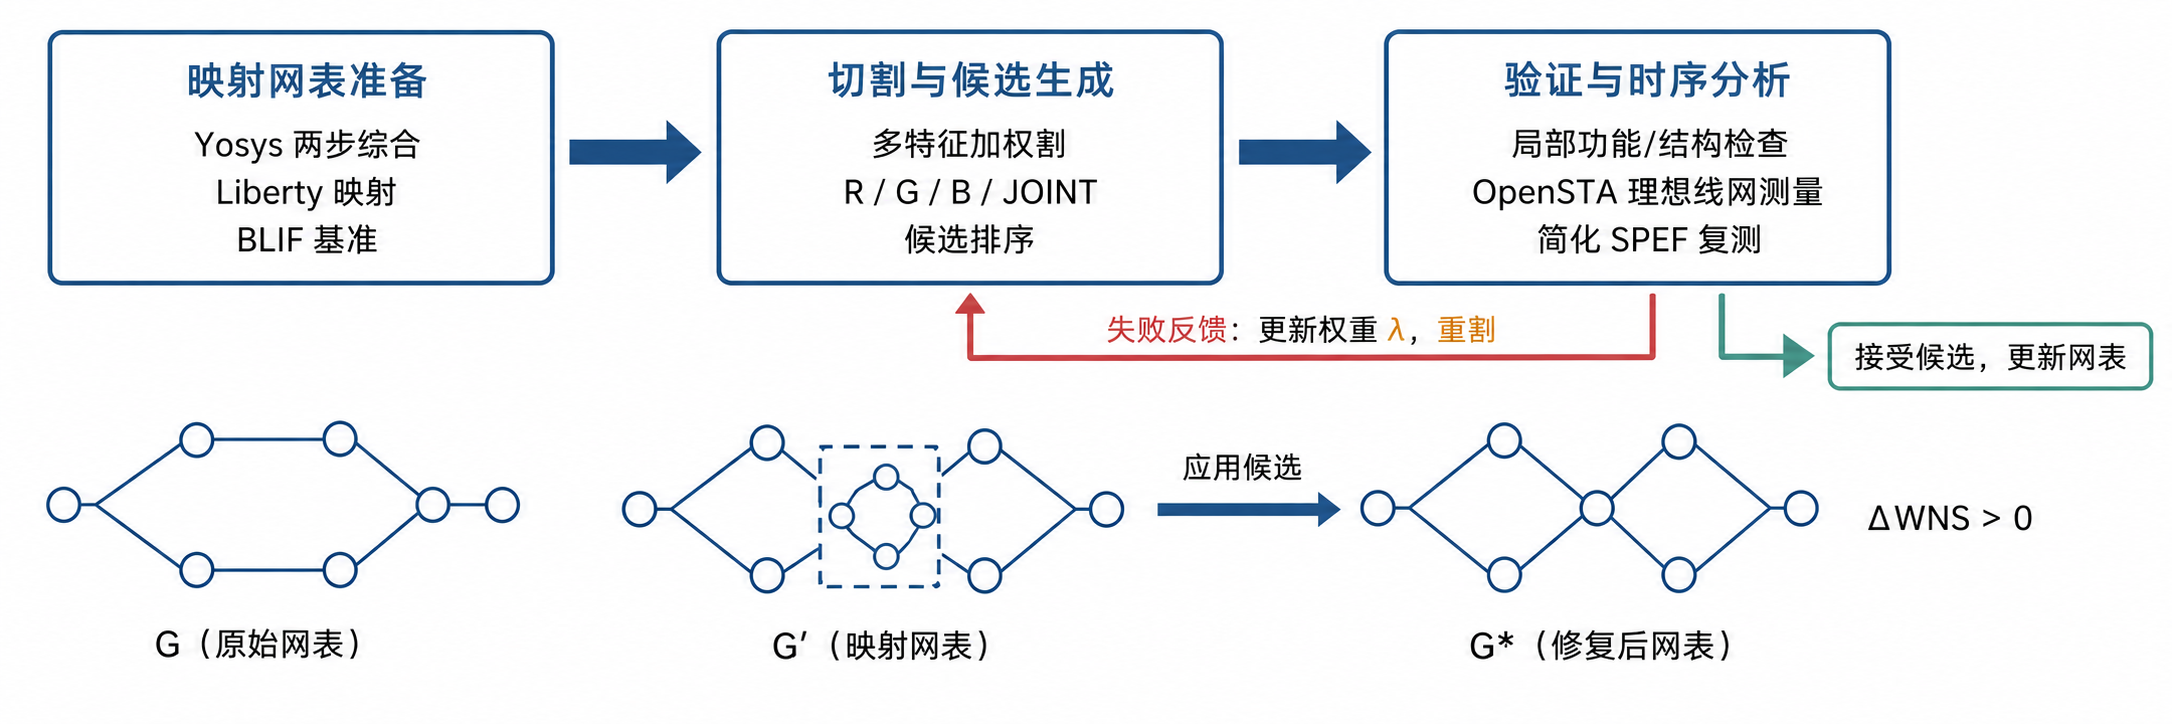
\includegraphics[width=0.96\columnwidth]{fig_method_flow_redraw_20260814.png}%
\caption{FAECO 三阶段流水线：映射网表准备 $\rightarrow$ 切割与候选细化 $\rightarrow$ 验证与时序分析。}
\label{fig:method_flow}
\end{figure}

\begin{algorithm}[H]
\footnotesize
\caption{FAECO 修复流程示意}\label{alg:main}
\begin{algorithmic}[1]
\Require 映射网表 $G'$、时序约束 $T$、工艺库 $\mathcal{L}$
\Ensure 修复后网表 $G^*$、接受候选集合 $\mathcal{A}$
\State 保存基线网表 $G_0\gets G'$，初始化当前网表 $N\gets G_0$、$G^*\gets G_0$、$\mathcal{A}\gets\emptyset$ 和搜索权重 $\lambda$
\Repeat
  \State 从\textbf{当前网表 $N$} 的最差违例端点提取扇入锥，必要时按深度分治
  \State 构建加权割与关键路径覆盖割，生成并排序 R/G/B/JOINT 候选
  \State 对候选执行局部功能/结构检查和 OpenSTA 测量
  \State 对满足物理门控条件的候选进行简化 SPEF 复测
  \State 若候选满足式~\eqref{eq:accept} 并在启用物理门控时通过简化 SPEF 复测，则将其加入 $\mathcal{A}$，并将该候选应用于当前网表、提交为下一轮评估基准（$N\gets N+\Delta$），同时更新最优网表 $G^*$。同一轮内多个候选共享同一基准 $N$ 且互不叠加；该轮一旦提交，基于旧基准的其余候选即作废，下一轮从提交后的网表重新提取违例端点与扇入锥并重新生成候选
  \State \textbf{若启用失效反馈控制}，触发 F1--F6 的失效候选按对应失效类型更新搜索参数；固定权重配置仅记录失效类型、不更新权重。因 10\,ps 阈值直接过滤的候选不参与失效反馈
\Until{无时序违例、候选耗尽或达到停止条件}
\State \Return $G^*,\ \mathcal{A}$
\end{algorithmic}
\end{algorithm}

算法~\ref{alg:main} 给出从违例端点提取扇入锥、生成候选、时序测量到反馈重搜索的流程。候选按轮提交：每轮接受的候选经验证后成为下一轮的评估基准，故多轮配置下修复网表由接受的补丁逐轮累积形成，效率优先配置（\S\ref{sec:eff_prio}）仅执行单轮；候选接受谓词与验证层次在 \S\ref{sec:validation} 中统一定义。

\subsection{加权割与候选搜索}\label{sec:mechanism}
\begin{figure*}[!tb]
\centering
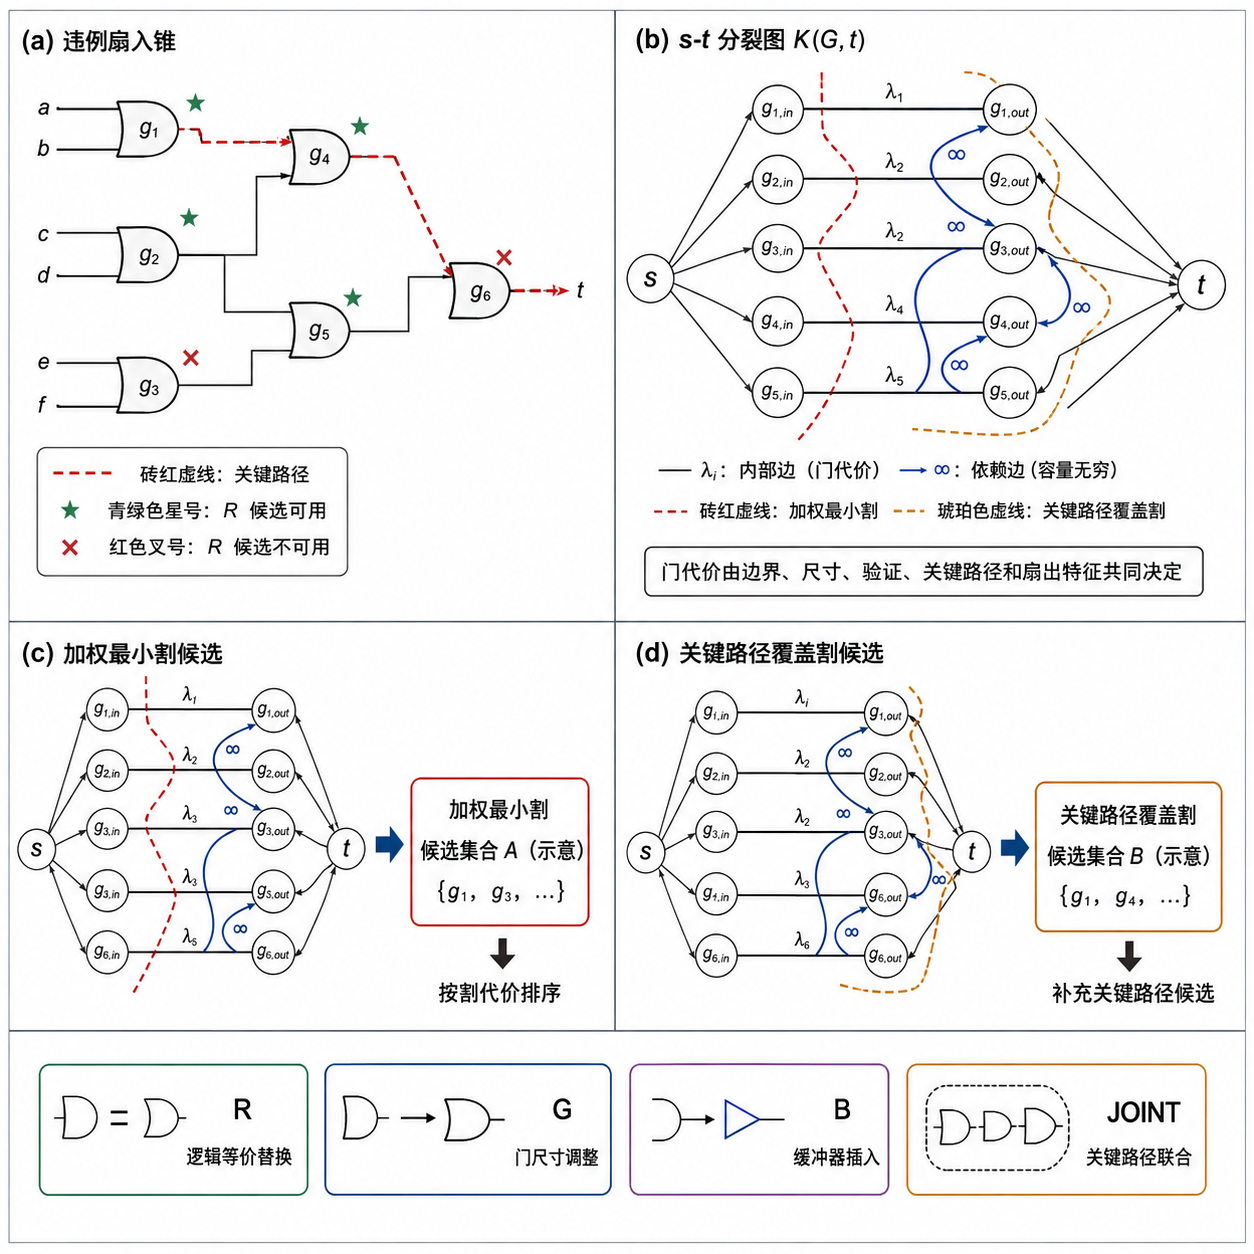
\includegraphics[width=0.65\textwidth]{fig_cut_generation_mechanism_imagegen.png}
\caption{FAECO 候选构造与排序机制：加权最小割控制候选规模，关键路径覆盖割 $C_c$ 补充时序关键候选，R 候选可用性参与策略切换；图中候选集合 A/B 分别对应 $C_w$ 与 $C_c$。}
\label{fig:cut_generation}
\end{figure*}

图~\ref{fig:cut_generation} 展示 FAECO 的核心原理。首先，从违例端点反向提取局部组合扇入锥 $C(G,t)$，并为门节点标注功能保持可用性、关键路径覆盖和候选规模等特征。加权最小割的节点代价由边界、候选规模、验证代价和扇出特征构成，并按权重 $\lambda_c$ 对具备 R 等价候选的门施加深度折扣，如式（2）所示；关键路径覆盖另通过独立的关键路径覆盖割 $C_c$ 形成补充候选，并由 $\lambda_c$ 反馈调整其排序优先级。R 候选的可用性用于候选实例化与策略切换——若某门缺少 R 等价候选，则其关键路径覆盖折扣与扇出代价同时失效并自动转向 G/B 策略。

随后，FAECO 生成两类互补边界：加权最小割 $C_w$ 优先控制局部规模，关键路径覆盖割 $C_c$ 覆盖时序关键门。两类边界分别实例化为 R/G/B/JOINT 候选，统一按割代价、关键路径覆盖和策略优先级排序，交由 OpenSTA 测量 $\Delta_{\mathrm{WNS}}$ 和 $\Delta_{\mathrm{TNS}}$。接受谓词保留有效候选；若启用失效反馈控制，触发 F1--F6 的失效候选按失效类型更新相应搜索权重，作为下一轮候选构造的控制输入，固定权重配置仅记录失效类型。该更新在本文中被定位为\textbf{搜索诊断与控制机制}，其是否带来独立增益由 \S\ref{sec:ablation} 单独检验。

候选 $p$ 的 WNS 改善量在相同 SDC 和时钟约束下定义为：
\begin{equation}\label{eq:dtiming}
\Delta_{\mathrm{WNS}}(p) = \mathrm{WNS}_{\mathrm{after}}(p) - \mathrm{WNS}_{\mathrm{before}}.
\end{equation}
节点代价 $\mathrm{cost}(v)$ 综合边界、尺寸、验证和扇出因素，并按关键路径深度折扣归一化。设 $\mathrm{depth}(v)$ 为 $v$ 在锥内的逻辑深度，$\mathcal{R}$ 为具备 R 等价候选的门集合，$\mathbb{1}[\cdot]$ 为指示函数，则
{\small
\begin{equation}
\label{eq:cost}
\begin{aligned}
\mathrm{cost}(v) ={}& \Big(1 + \frac{\lambda_b}{1+\mathrm{depth}(v)}
 + \lambda_s\,\frac{s(v)^2}{S}
 + 0.01\lambda_v\,n_C \\
 &+ 0.1\lambda_f\,\mathbb{1}[v{\in}\mathcal{R}]\,\mathrm{fanout}(v)\Big) \\
 &\Big/\Big(1 + \lambda_c\,\mathbb{1}[v{\in}\mathcal{R}]\,
 \frac{\mathrm{depth}(v)}{\mathrm{depth}_{\max}}\Big),
\end{aligned}
\end{equation}
}
其中 $\lambda_b/\lambda_s/\lambda_v/\lambda_f$ 分别为边界、尺寸、验证和扇出权重，$\lambda_c$ 为关键路径深度折扣权重，默认均为 $1.0$；$n_C=|C(G,t)|$ 为目标扇入锥的门数，$s(v)$ 为门 $v$ 的局部扇入锥规模，$S=\sum_u s(u)^2$，$\mathrm{depth}_{\max}=\max_u \mathrm{depth}(u)$。扇出项与分母折扣均以 $\mathbb{1}[v{\in}\mathcal{R}]$ 为门控：缺少 R 等价候选的门不可重写，若仍被深度折扣，只会把不可重写的门推入候选边界并最终触发 F1 失效，故对这类门同时免除扇出代价与深度折扣。$\lambda_c$ 同时参与关键路径覆盖候选的排序，用于调节对高关键度节点的偏好；归一化项用于抑制大锥规模。其中 $0.01$ 与 $0.1$ 为固定的特征尺度系数，分别作用于验证代价项（随锥门数 $n_C$ 增长）与扇出项（随扇出数增长），使其与式中其余无量纲项保持可比量级；二者在实现中为固定常量，所有实验均保持不变。

\subsection{类型化失效归因与搜索控制}

\FloatBarrier
框架将 F1--F6 定义为统一的候选失效类型，用于对候选验证结果进行结构化归因：真实 WNS 主循环中观测到的主要类型为 F4（理想线网收益不足），启用物理门控时进一步将 SPEF 复测失效记为 F6，各类检测条件见表~\ref{tab:failures}。启用失效反馈控制时，按表~\ref{tab:failures} 的对应动作调整搜索参数（每类失效使相应权重增加 $1.0$，F5 额外将最大锥门数减半），固定权重配置仅记录失效类型。F6 记录简化 SPEF 复测下的物理失效，并可在启用反馈控制时参与搜索参数更新；本文主要验证其候选识别与过滤作用，尚未证明该反馈能够独立提高最终物理 WNS，见 \S\ref{sec:phys_closure}。本文另实现以指数滑动平均（EMA）平滑的自适应更新，并仅在 \S\ref{sec:ablation} 中作为消融对象。

\begin{table}[!htbp]
\centering
\caption{F1--F6 失效类型与搜索控制动作}
\label{tab:failures}
\scriptsize
\setlength{\tabcolsep}{2pt}
\begin{tabular}{p{2.0cm}p{2.6cm}p{2.9cm}}
\toprule
\textbf{失效类型} & \textbf{检测条件} & \textbf{控制动作} \\
\midrule
F1 局部功能/结构失效 & Liberty 文件中的函数匹配或结构检查未通过 & 增加边界惩罚 $\lambda_b$ 与扇出权重 $\lambda_f$（抑制高扇出的不稳定等价点），降低此类节点被选作候选边界的概率 \\
F2 边界失效 & 锥边界未闭合 & 增加边界惩罚 $\lambda_b$，收紧锥边界，保留已映射门 \\
F3 尺寸过大 & 候选尺寸超过阈值 & 增加尺寸惩罚，强制更小割 \\
F4 时序收益不足 & 候选未满足式~\eqref{eq:accept} & 上调关键路径深度折扣 $\lambda_c$（同时提高覆盖割排序优先级），使下一轮割集方案集中于真实关键路径门 \\
F5 验证超时 & 局部检查或 STA 运行时间 $>60\,$s & 增加验证代价惩罚 $\lambda_v$ 并将最大锥门数减半 \\
F6 SPEF 复测失效 & 启用物理门控且理想线网增益 $>10\,$ps，但 SPEF 下 WNS 不改善 & 增加边界惩罚 $\lambda_b$，收紧候选边界并偏向较小局部 \\
\bottomrule
\end{tabular}
\end{table}

\subsection{验证与接受}\label{sec:validation}
候选验证分为构造筛选、时序测量和最终等价验证三个层次。R 候选由 Liberty 函数匹配生成，G/B 候选由保持逻辑函数的局部结构变换生成；组合网表可在启用相应流程时由 ABC \texttt{cec} 回验。主实验和跨测试集实验对最终基线网表与修复网表执行独立顺序 SEC，SEC 结果与理想线网 WNS 候选接受判定分开统计。该 SEC 在 SKY130 行为单元模型下验证组合逻辑与状态转移关系；理想线网 WNS 和 OpenROAD 全局布线寄生估计后的 WNS 分别由 OpenSTA 与 OpenROAD 流程测量。

候选 $p$ 在相同 SDC、时钟约束和分析角下的接受谓词为
\begin{equation}
\label{eq:accept}
\begin{aligned}
A(p)={}&[\Delta_{\mathrm{WNS}}(p)>0]\\
&\lor[\mathrm{tns\_aware}\land\Delta_{\mathrm{WNS}}(p)=0\\
&\qquad\land\Delta_{\mathrm{TNS}}(p)>0].
\end{aligned}
\end{equation}
启用物理门控时，满足式~\eqref{eq:accept} 且理想线网增益超过 10\,ps 的候选进一步接受简化 SPEF 复测；$0<\Delta\mathrm{WNS}\le10\,$ps 的候选不进入最终接受集合。复测下 WNS 仍改善的候选进入接受集合 $\mathcal{A}$，否则记为 F6；启用失效反馈控制时该失效用于下一轮搜索参数更新，固定权重配置仅记录该失效。未启用物理门控时，SPEF 结果作为独立物理复测，不改变理想线网候选的接受判定。

\FloatBarrier
\subsection{复杂度}\label{sec:impl}

分裂图采用最大流—最小割求解。若锥内门数为 $n$、扇入依赖边数为 $f$，则分裂图节点数为 $V=2n+2$、边数为 $E=O(n+f)$；采用 Edmonds--Karp 求解时，单次割求解复杂度为 $O(VE^2)$。具体工具版本、运行环境和参数配置见第~\ref{sec:setup} 节。

扇入锥 $C(G, t) = (V_C, E_C)$ 由反向广度优先搜索（BFS）抽取。对大规模设计，按逻辑深度将违例锥切分为受门数上限约束的子锥，独立生成候选并沿关键路径排序，以控制内存和求解规模。

% =============================================================================
% IV. 实验
% =============================================================================
\FloatBarrier
\section{实验}\label{sec:exp}

\subsection{实验设置}\label{sec:setup}

\textbf{环境与数据集}：实验在 WSL2 Ubuntu 上完成，主流程采用 OSS-CAD Suite（Yosys 0.67+146、OpenSTA 3.1.0），顺序 SEC 采用 WSL 环境中的 Yosys 0.33。测试集包含 8 个 ISCAS89、19 个 ITC-99 和 3 个 PicoRV32 子模块，统一使用 0.5 ns 时钟约束。\textbf{0.5 ns 作为统一的 stress-test timing constraint 而非各设计的目标工作频率，用以保证不同 benchmark 均产生可供候选搜索比较的 setup violation；本文关注的是固定约束下的相对 WNS 改善，不等同于 timing closure。}主要评价指标为 WNS、全局布线寄生估计后的 WNS 和候选级 STA 次数；TNS 用于可选的辅助接受判据。本文以 WNS 严格改善作为主要效果统计口径。跨测试集实验中，b06 保留 WNS 持平且 TNS 改善时的辅助接受条件；该类补丁不计入“严格 WNS 改善”统计。其余实验以 WNS 严格改善为主要接受条件；TNS-aware 仅作为可选扩展，不与本文物理门控实验联合启用。

\textbf{benchmark 纳入规则}：ISCAS89 纳入能够经统一 Yosys→SKY130 HD 流程成功映射并形成有效 setup timing path 的 8 个顺序电路；ITC-99 按相同标准纳入 19 个电路（b01--b15、b17、b20--b22），其中 b18、b19 未纳入上述统一统计，在相同流程下作为大规模补充实例单独运行并报告（见 \S\ref{sec:itc99}）；PicoRV32 选择主核 \texttt{picorv32}、乘法协处理器 \texttt{picorv32\_pcpi\_mul} 与存储密集子模块 \texttt{picorv32\_regs}（存储簇）以覆盖控制、算术和存储三类结构差异。

\textbf{实验配置}：为避免不同搜索预算和实现版本造成混淆，\S\ref{sec:iscas}--\S\ref{sec:s_boundary} 分别采用各自固定的实验配置，各小节结果仅在对应配置内比较，不跨配置合并统计。其中 \S\ref{sec:iscas} 为效率优先配置（单轮、首改进即停、仅轮内失效反馈，见表~\ref{tab:configs}），源于早期冻结结果并独立报告；\S\ref{sec:ood}、\S\ref{sec:ablation} 与 \S\ref{sec:s_boundary} 使用后续统一实验流程，分别用于跨测试集评估（三组 benchmark 同一批运行，最多 8 轮）、候选空间与排序消融（固定 20 轮预算）以及结构候选能力边界（开关对照）；\S\ref{sec:phys_closure} 包含两类独立的物理验证：OpenROAD 后验验证使用 \S\ref{sec:iscas} 的接受候选，SPEF 负载扫描与门控实验单独报告。b17 的验证时限例外见 \S\ref{sec:itc99}。完整脚本和参数随补充材料一同发布。

\begin{table}[!htb]
\centering
\caption{效率优先与 20 轮收敛配置的关键参数对比}
\label{tab:configs}
\scriptsize
\setlength{\tabcolsep}{4pt}
\begin{tabular}{lcc}
\toprule
\textbf{参数} & \textbf{效率优先} & \textbf{20 轮收敛} \\
\midrule
最大迭代轮数                    & 1（首改进即停止） & 20 \\
F1--F6 失效反馈                  & 仅轮内 & 不启用（固定权重） \\
10\,ps 物理门控 SPEF 复测        & 关 & 关 \\
单候选验证时限（默认）           & 60\,s & 60\,s \\
\bottomrule
\multicolumn{3}{p{0.95\columnwidth}}{\footnotesize 注：20 轮收敛配置（\S\ref{sec:ablation}）各列由固定权重运行器产生，用于比较候选空间与候选排序；跨测试集主实验（\S\ref{sec:ood}）最多迭代 8 轮、启用跨轮失效反馈，其余关键参数与效率优先配置相同；b17 的验证时限例外（180\,s）属跨测试集实验（\S\ref{sec:itc99}）。}\\
\end{tabular}
\end{table}

\textbf{接受准则}：除 \S\ref{sec:itc99} 所述 b06 的 TNS 辅助接受外，其余主实验均以式~\eqref{eq:accept} 的 WNS 严格改善为主要接受条件；本文不将“取得 WNS 改善”等同于 timing closure。

\subsection{效率优先子研究：ISCAS89 修复质量与效率}\label{sec:iscas}

本小节报告 \S\ref{sec:setup} 所述效率优先子研究在 ISCAS89 上的结果。

图~\ref{fig:iscas_main} 所示的 8 个 ISCAS89 基线网表与修复网表的对比结果，在预布局理想线网模式下经 OpenSTA 测量均实现严格改善；修复候选来自不改写 D 触发器、时钟和复位的 R/G/B/JOINT 构造级保持变换。本子研究的 8 个电路均通过独立顺序 SEC（通过率 8/8），证明单元数和时间见表~\ref{tab:sec_iscas8}。接受的候选类型分布为 JOINT 4 个（s27/s382/s420/s953）、G 3 个（s641/s713/s832）、R 1 个（s820），由各电路候选调用台账中被接受 trial 的类型字段给出；B 策略不纳入本组建立时间对比结果。\textbf{图~\ref{fig:iscas_main} 对应效率优先配置}\label{sec:eff_prio}，该配置\textbf{不启用 §3.5 的 10\,ps 物理门控阈值}，直接以式~\eqref{eq:accept} 的 WNS$>0$ 为接受准则，因此 s420 的 +0.01\,ns（10\,ps）接受候选不与 §3.5 的过滤规则冲突。

\textbf{来源说明}：该子研究来源于早期冻结结果，当前版本按相同公开配置重跑仍保持 8/8 严格改善，但部分搜索路径发生变化，因此本文仅将其作为独立的效率子研究，不与后续统一实验流程合并统计。

从机制上看，JOINT 联合多个局部变换，能够同时调整局部实现与驱动条件；G 主要改变驱动强度，R 则受工艺库中等价布尔实现的可用性限制。

\begin{figure}[!t]
\centering
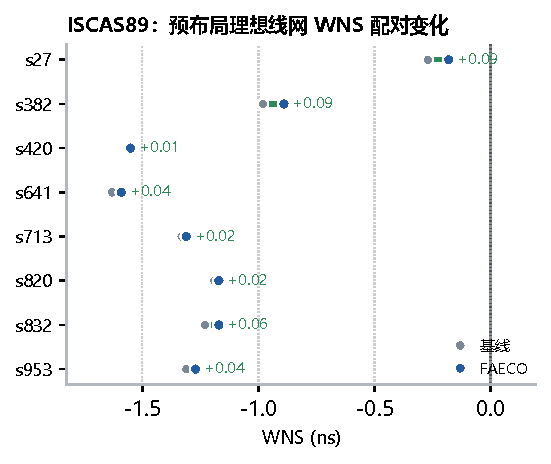
\includegraphics[width=1.0\columnwidth]{fig_iscas89.pdf}
\caption{ISCAS89 顺序电路混合修复的基线与 FAECO 结果对比（周期 0.5 ns；标注为 FAECO 相对基线的 WNS 变化）}
\label{fig:iscas_main}
\end{figure}

\begin{table}[!htb]
\centering
\caption{ISCAS89 顺序门级 SEC 结果}
\label{tab:sec_iscas8}
\setlength{\tabcolsep}{4pt}
\footnotesize
\begin{tabular}{lrrr}
\toprule
\textbf{电路} & \textbf{$\mathrm{equiv}$ 单元} & \textbf{SEC} & \textbf{时间 (s)} \\
\midrule
s27  & 11  & 通过 & 0.303 \\
s382 & 90  & 通过 & 0.382 \\
s420 & 79  & 通过 & 0.368 \\
s641 & 124 & 通过 & 0.381 \\
s713 & 126 & 通过 & 0.410 \\
s820 & 138 & 通过 & 0.454 \\
s832 & 145 & 通过 & 0.437 \\
s953 & 228 & 通过 & 0.537 \\
\bottomrule
\multicolumn{4}{p{0.92\columnwidth}}{\footnotesize 使用 \texttt{equiv\_make} + \texttt{equiv\_simple} + \texttt{equiv\_induct} 进行证明；8 个电路共 8/8 通过。该结果对应 SKY130 行为单元模型下的逻辑门级顺序等价证明。}\\
\end{tabular}
\end{table}

\FloatBarrier
\subsection{跨测试集评估}\label{sec:ood}

\subsubsection{ITC-99 基准族}\label{sec:itc99}

在纳入统一批量评估的 19 个 ITC-99 电路中，18 个电路的 WNS 取得严格改善，b06 与基线持平（$\Delta = 0\,\text{ns}$），19 个电路均无 WNS 回退。b17 在默认 60\,s 单候选验证时限下所有候选均触发 F5 超时而被拒，将其单候选验证时限放宽至 180\,s（其余 18 个电路仍用默认）后，在 104 次候选级 STA 测量内取得 $+0.38\,$ns 改善（接受 G 候选 nor4b$_1\!\to\!$nor4b$_2$）。纳入统计的大规模电路 b14/b15/b17/b20/b21/b22 均取得严格 WNS 改善。b06 的基线 WNS 为 $-0.56\,\text{ns}$，其关键路径包含多个相邻的 \texttt{or4b$_1$}，G 策略因增大输入电容拖累前级、B 策略无可缓解的低扇出网络、R 候选在 SKY130 HD 库中无等价族；混合 R/G/B/JOINT 共 664 次候选级 STA 测量中无一次严格超过基线，表明 b06 在当前搜索空间中的进一步改善受限。

接受补丁以 G 为主力：19 个电路中 17 个含 G 类接受（累计 69 次），B 与 R 类接受分别出现于 14 个和 10 个电路；收益最大的 b20/b21（分别为 $+1.98$ 和 $+2.75\,\text{ns}$）均以 G 为主、辅以 R。19 个电路共进行 3363 次候选级 STA 测量。19 个电路改善量的中位数为 $+0.18\,\text{ns}$、均值为 $+0.43\,\text{ns}$，均值由 b20/b21 大电路（基线 WNS $\le -13\,\text{ns}$）拖高，本文同时报告中位数与均值。

作为大规模补充实例（未纳入上述 19 个电路的统一统计）：b18（SKY130 映射后 7.57 万个单元）的 WNS 在 0.5 ns 下由 $-13.34$ ns 改善至 $-13.27$ ns，经 24 次候选级 STA 测量完成修复；b19（15.10 万个单元）由 $-17.44$ ns 改善至 $-16.00$ ns，经 59 次完成。

\subsubsection{PicoRV32 异构族}

基于同一寄存器传输级（RTL）源的三个结构差异明显的子模块直接复用 ISCAS89 流程：PicoRV32 主核与其 PCPI 乘法协处理器 \texttt{picorv32\_pcpi\_mul} 分别获得 $+1.13$ 和 $+0.07\,$ns 的改善（修复网表由 R/G/B 多类接受补丁叠加形成），存储密集子模块 \texttt{picorv32\_regs} 为存储簇、无可建立 setup 路径，未纳入改善统计。

统一跨测试集评估中，三组数据集的 WNS 严格改善比例分别为 8/8、18/19 和 2/3。顺序 SEC 面向 30 个测试实例：29 个实例产生实际网表修改，其中 28/29 个修改网表对完全证明（三组分别为 8/8、18/19 和 2/2）；b06 的最终 WNS 与基线持平，其接受的缓冲器/延迟单元补丁不改变 WNS，并经顺序 SEC 完全证明；唯一未产生接受补丁的 \texttt{picorv32\_regs} 无 setup 路径，其输出网表与基线一致。b17 的修复网表经 Yosys \texttt{equiv\_simple} + \texttt{equiv\_induct} 验证 12812 个等价点，仅剩 1 个未证明点（nor4b$_1\!\to\!$nor4b$_2$ 的同函数尺寸替换，Liberty function 一致），本文将其单独报告。

\subsection{候选空间、排序与反馈消融}\label{sec:ablation}

本节分两组实验。首先，在相同 20 轮预算与固定权重下（表~\ref{tab:ablation} 四列均不含 F1--F6 权重重整，故不构成失效反馈的开关对照）比较候选空间与候选评估顺序：混合候选空间的平均 WNS 改善为 1.07\,ns，在 8/8 个电路上高于纯 G（均值 0.16\,ns）、在 7/8 个上高于纯 B（均值 0.54\,ns）。保持候选空间不变、仅随机化每轮评估顺序后，平均改善降为 0.40\,ns，且 s713、s953 取得首个改进所需的候选级 STA 次数分别由 5、1 增至 216、185，说明结构化排序对搜索效率具有明显作用。其次，保持候选空间和初始排序条件不变，对比 Fixed 与 Adaptive 以单独检验失效反馈自适应的作用：两者在 8/8 个电路上的最终 $\Delta\mathrm{WNS}$、首次改善位置和最大 $B(k)$ 均一致；因此未观察到 EMA 更新带来的独立收益，本文不将该自适应反馈作为独立性能贡献，而是把 F1--F6 定位为搜索诊断与控制信号。

\begin{table}[H]
\centering
\caption{ISCAS89 候选空间与候选排序设置的 WNS 改善对比（周期 0.5\,ns）}
\label{tab:ablation}
\scriptsize
\setlength{\tabcolsep}{3pt}
\begin{tabular}{lrrrr}
\toprule
\textbf{电路} & \textbf{纯 G} & \textbf{纯 B} & \textbf{随机} & \textbf{混合 20 轮} \\
\midrule
s27  & +0.09 & +0.28 & +0.28 & \textbf{+0.28} \\
s382 & +0.17 & +0.19 & +0.19 & \textbf{+1.00} \\
s420 & +0.35 & +1.00 & +1.15 & \textbf{+1.54} \\
s641 & +0.45 & +1.27 & +0.57 & \textbf{+1.63} \\
s713 & +0.05 & +0.99 & +0.64 & \textbf{+1.33} \\
s820 & +0.02 & +0.26 & +0.15 & \textbf{+0.99} \\
s832 & +0.07 & +0.06 & +0.08 & \textbf{+0.57} \\
s953 & +0.09 & +0.24 & +0.12 & \textbf{+1.25} \\
\midrule
\textbf{均值} & 0.16 & 0.54 & 0.40 & \textbf{1.07} \\
\bottomrule
\multicolumn{5}{p{0.92\columnwidth}}{\footnotesize 数字为 WNS 改善量 (ns)，正值代表修复后 WNS 较基线提高。纯 G / 纯 B 列为单策略候选空间；随机列与混合 20 轮列为混合候选空间，随机列每轮随机化候选评估顺序并取种子 1、2、3 的均值。四列均为固定搜索权重、不启用 F1--F6 权重重整，采用式~\eqref{eq:accept} 与相同的 20 轮上限和候选评估预算，故本表量化候选空间与候选排序的贡献。} \\
\end{tabular}
\end{table}

\subsection{物理估计与诊断}\label{sec:phys_closure}
\FloatBarrier

本节物理验证采用 \S\ref{sec:eff_prio} 效率优先配置得到的接受候选，与 \S\ref{sec:ablation} 的 20 轮收敛配置分开统计。表~\ref{tab:pr8} 首先对 \S\ref{sec:eff_prio} 效率优先配置得到的接受候选进行后验 OpenROAD 物理估计验证。在 OpenROAD 2.0 布局与全局布线（global routing）寄生估计后，8 个 ISCAS89 电路中有 5 个电路保持时序改善，1 个持平，2 个轻微恶化但不超过 0.02 ns。流程使用 OpenROAD 2.0、SKY130 HD 和 0.5 ns 时钟约束。另行开展 SPEF 负载扫描与门控实验，用于观察候选对线载估计的敏感性，并记录 F6 失效。

\FloatBarrier

独立 SPEF 负载扫描显示，s382 的 R 候选与 b18 的 JOINT 候选的 WNS 改善随估计线长增大而归零，表明线载增大后理想线网收益逐步衰减。

\textbf{迭代式门控}：在 40\,$\mu$m/unit 估计线载下（unit 表示一次扇出后沿拓扑/曼哈顿距离累加的相对单位长度），对每条线 $e$ 用简化公式 $L_{\mathrm{est}}(e)=40\,\mu\mathrm{m} \cdot u(e)$、$R_e=r_{\mathrm{unit}}L_{\mathrm{est}}$、$C_e=c_{\mathrm{unit}}L_{\mathrm{est}}$ 估计寄生电阻电容（$r_{\mathrm{unit}}$、$c_{\mathrm{unit}}$ 取自 SKY130 HD \texttt{li1} 层代表 RC），并据此生成简化 SPEF。s382 的 50 个和 b18 的 6 个候选均未通过 SPEF 复测，并被记录为 F6；在启用反馈控制的配置中，相应失效用于更新搜索参数。该实验能够证明 F6 可识别并拒绝 ideal-net 下有效而在线载后失效的候选，但尚不能证明其反馈能够改善最终物理 WNS。

\FloatBarrier

\begin{table}[ht]
\centering
\caption{OpenROAD 布局及全局布线寄生估计后的 WNS 对比（8 个 ISCAS89 电路）}
\label{tab:pr8}
\footnotesize
\setlength{\tabcolsep}{2pt}
\begin{tabular}{lrrrrr}
\toprule
 & \multicolumn{2}{c}{\textbf{预布局}} & \multicolumn{2}{c}{\textbf{全局布线估计}} & \\
\cmidrule(lr){2-3}\cmidrule(lr){4-5}
\textbf{电路} & \textbf{基线} & \textbf{修复} & \textbf{基线} & \textbf{修复} & $\Delta$ \\
\midrule
s27  & $-0.27$ & $-0.18$ & $-0.36$ & $-0.22$ & $+0.14$ \\
s382 & $-0.98$ & $-0.89$ & $-1.16$ & $-1.02$ & $+0.14$ \\
s420 & $-1.56$ & $-1.55$ & $-1.80$ & $-1.82$ & $-0.02$ \\
s641 & $-1.63$ & $-1.59$ & $-2.10$ & $-2.02$ & $+0.08$ \\
s713 & $-1.33$ & $-1.31$ & $-1.59$ & $-1.58$ & $+0.01$ \\
s820 & $-1.19$ & $-1.17$ & $-1.52$ & $-1.49$ & $+0.03$ \\
s832 & $-1.23$ & $-1.17$ & $-1.51$ & $-1.51$ & $0.00$ \\
s953 & $-1.31$ & $-1.27$ & $-1.60$ & $-1.61$ & $-0.01$ \\
\bottomrule
\multicolumn{6}{p{0.92\columnwidth}}{\footnotesize 各电路物理估计采用与预布局评估一致的映射网表及接受候选；s27 采用 10\% 利用率布局规划；$\Delta$ 为全局布线寄生估计后修复网表相对基线的 WNS 变化。}\\
\end{tabular}
\end{table}

\FloatBarrier
\subsection{结构候选扩展与能力边界}\label{sec:s_boundary}
\FloatBarrier

除 R/G/B/JOINT 构造级变换外，本文还实现了一类窗口局部结构重综合候选（记为 S），用于检验“更深的结构改写”能否成为新的修复能力来源。为排除“枚举宽度不足”这一因素，我们对 S 的窗口池单独扩池并做开关对照：控制臂（S 关）在 8/8 个电路上与既有结果逐位一致，两臂的非 S 候选序列一致，候选级 STA 预算未触及上限。

\begin{table}[H]
\centering
\caption{结构候选（S）的能力边界}
\label{tab:s_boundary}
\footnotesize
\setlength{\tabcolsep}{8pt}
\begin{tabular}{lrr}
\toprule
\textbf{指标} & \textbf{原配置} & \textbf{扩池} \\
\midrule
S 候选数 & 37 & 126 \\
$\Delta L>0$ & — & 76/126 \\
$\Delta_{\mathrm{WNS}}>0$ & 0 & 0/126 \\
$\Delta_{\mathrm{WNS}}<0$ & — & 90/126 \\
接受电路 & 0/8 & 0/8 \\
\bottomrule
\multicolumn{3}{p{0.9\columnwidth}}{\footnotesize $\Delta L=L_{\mathrm{before}}-L_{\mathrm{after}}$，正值表示 SKY130 映射后逻辑深度降低；$\Delta_{\mathrm{WNS}}=\mathrm{WNS}_{\mathrm{after}}-\mathrm{WNS}_{\mathrm{before}}$，正值表示时序改善。扩池仅在窗口来源侧生效，不改变接受谓词与验证流程。}\\
\end{tabular}
\end{table}

扩池后 S 候选由 37 增至 126，其中 76 个候选降低了 SKY130 映射后的逻辑深度，但无候选取得严格 WNS 改善，90 个候选反而使 WNS 恶化，8 个电路均未接受 S 候选。因此，在本文评测的窗口构造、重综合、映射流程和基准集合下，S 的限制已不能归因于枚举宽度不足；逻辑深度降低也未转化为端到端时序收益。进一步扩大枚举池不能解释或解决当前 S 候选的时序收益不足，本文将其保留为可选候选类型。

\FloatBarrier
\section{结论}\label{sec:conclusion}

本文提出 FAECO，一种面向预布局门级时序 ECO 的结构化候选搜索与失效归因框架，其核心由三部分组成：在违例扇入锥上以多特征加权割与关键路径覆盖割生成 R/G/B/JOINT 候选，并按割代价、关键路径覆盖与策略优先级完成结构化排序；将候选失效归为 F1--F6 六类用于失效归因与搜索控制；候选按轮提交，经理想线网 STA、简化 SPEF 复测与独立顺序 SEC 分层验证。

在统一的跨测试集评估中，FAECO 在 ISCAS89、ITC-99 和 PicoRV32 上分别实现 8/8、18/19 和 2/3 个电路的严格 WNS 改善（仅指 WNS 改善，不等同于 timing closure）。固定权重、20 轮上限的对比显示，混合候选空间的平均 WNS 改善为 1.07\,ns、纯 G 为 0.16\,ns，且随机化评估顺序会使首个改进所需的候选级 STA 次数恶化 1--2 个数量级，表明候选空间与结构化排序对搜索收益和搜索效率具有明确贡献。

本文同时明确两项能力边界：以失效类型更新权重的 EMA 自适应与固定权重在 8/8 个电路上结果一致，未表现出独立收益，故仅作为可选机制保留（\S\ref{sec:ablation}）；窗口局部结构重综合候选在解除枚举上限后仍未产生正 WNS 增益，保留为可选候选类型（\S\ref{sec:s_boundary}）。OpenROAD 布局及全局布线寄生估计后，5 个 ISCAS89 电路保持改善、1 个持平，2 个退化不超过 0.02\,ns。



\renewcommand{\refname}{参考文献}
\ctexset{section = {format=\heiti\fontsize{10.5}{14}\selectfont}}
\footnotesize
\linespread{0.95}\selectfont
\balance
\begin{thebibliography}{99}
\bibitem{ho2010eco} Ho K H, Chen Y P, Fang J W, et al. ECO timing optimization using spare cells and technology remapping[J]. IEEE Transactions on Computer-Aided Design of Integrated Circuits and Systems, 2010, 29(5): 697-710. DOI: 10.1109/TCAD.2010.2043573.
\bibitem{liu2021rlsizer} Lu Y C, Nath S, Khandelwal V, et al. RL-Sizer: VLSI gate sizing for timing optimization using deep reinforcement learning[C] //Proceedings of the 58th ACM/IEEE Design Automation Conference. Piscataway: IEEE, 2021: 733-738. DOI: 10.1109/DAC18074.2021.9586138.
\bibitem{chen2024aito} Wu H, Huang Z, Li X, et al. AiTO: Simultaneous gate sizing and buffer insertion for timing optimization with GNNs and RL[J]. Integration, the VLSI Journal, 2024, 98: 102211. DOI: 10.1016/j.vlsi.2024.102211.
\bibitem{iscas89} Brglez F, Bryan D, Kozminski K. Combinational profiles of sequential benchmark circuits[C] //Proceedings of IEEE International Symposium on Circuits and Systems. Piscataway: IEEE, 1989: 1929-1934. DOI: 10.1109/ISCAS.1989.100747.
\bibitem{itc99} Davidson S. ITC'99 benchmark circuits - preliminary results[C] //Proceedings of IEEE International Test Conference. Piscataway: IEEE, 1999: 1125. DOI: 10.1109/TEST.1999.805857.
\bibitem{kravets2019symbolic} Kravets V N, Lee N Z, Jiang J H R. Comprehensive search for ECO rectification using symbolic sampling[C] //Proceedings of the 56th Annual Design Automation Conference. New York: ACM, 2019: 71:1-71:6. DOI: 10.1145/3316781.3317790.
\bibitem{jiang2010fraig} Wu B H, Yang C J, Huang C Y, et al. A robust functional ECO engine by SAT proof minimization and interpolation techniques[C] //Proceedings of IEEE/ACM International Conference on Computer-Aided Design. Piscataway: IEEE, 2010: 729-734. DOI: 10.5555/2133429.2133584.
\bibitem{jiang2016resource} Cheng A C, Jiang I H R, Jou J Y. Resource-aware functional ECO patch generation[C] //Proceedings of the Design, Automation \& Test in Europe Conference \& Exhibition. Piscataway: IEEE, 2016: 1036-1041. DOI: 10.5555/2971808.2972050.
\bibitem{zhong2024stp} Pan H, Zhang R, Xia Y, et al. A semi-tensor product based circuit simulation for SAT-sweeping[C] //Proceedings of the Design, Automation \& Test in Europe Conference \& Exhibition. Piscataway: IEEE, 2024: 1-6. DOI: 10.23919/DATE58400.2024.10546678.
\bibitem{zhuo2018patch} Dao A Q, Lee N Z, Chen L C, et al. Efficient computation of ECO patch functions[C] //Proceedings of the 55th Annual Design Automation Conference. New York: ACM, 2018: 1-6. DOI: 10.1145/3195970.3196039.
\bibitem{huang2025phys} Ye Y, Xu P, Ren L, et al. Learning-driven physically aware large-scale circuit gate sizing[J]. IEEE Transactions on Computer-Aided Design of Integrated Circuits and Systems, 2025, 44(5): 1901-1914. DOI: 10.1109/TCAD.2024.3488577.
\bibitem{zhang2025buffalo} Hsiao H H, Lu Y C, Lim S K, et al. BUFFALO: PPA-configurable, LLM-based buffer tree generation via group relative policy optimization[C] //Proceedings of IEEE/ACM International Conference on Computer-Aided Design. Piscataway: IEEE, 2025: 1-9. DOI: 10.1109/ICCAD66269.2025.11240744.
\bibitem{openroad} Ajayi T, Chhabria V A, Fogaça M, et al. Toward an open-source digital flow: First learnings from the OpenROAD project[C] //Proceedings of the 56th ACM/IEEE Design Automation Conference. New York: ACM, 2019: 1-4. DOI: 10.1145/3316781.3326334.
\bibitem{abc} Brayton R, Mishchenko A. ABC: An academic industrial-strength verification tool[C] //Proceedings of the 22nd International Conference on Computer Aided Verification. Berlin: Springer, 2010: 24-40. DOI: 10.1007/978-3-642-14295-6\_5.
\end{thebibliography}

\end{document}
